\chapter{Background Estimate}

This chapter discuses methods used to estimate background processes the the signal. These background processes can be split up in to two categories; Reducible and irreducible. Irreducible backgrounds consist of those background almost indistinguishable from our signal process namely clean high energy dielectron decays such as decays of the Z boson and the Drell-Yan (DY) spectrum. DY ($q\bar{q}~\rightarrow~Z/\gamma^{*}~\rightarrow~\ell^{-}\ell^{+}$) is largest background process and also interferes with the signal processes. Another irreducible background also estimated is the Photon Induced processes ($\gamma\gamma~\rightarrow~\ell^{-}\ell^{+}$) coming from the collision of two photons. Reducible backgrounds are those that can be reduced through event selection and three are included in this analysis. These reducible backgrounds consist of Top precessed, collisions creating single top quarks and $t\bar{t}$ events which decay to include two electrons, Diboson events, the creation of WW, WZ and ZZ events that decay in to two electron events, and finally Multi-jet \& W+jets events where one or more electron signature is faked by jet objects. All of these backgrounds are estimated via Monte Carlo generators except for the Multi-jet \& W+jets background which is estimated via a data-driven fake factor method. Once completed all background samples are summed together to create the full background estimate. MC samples are then scaled to the integrated luminosity of data collected in 2012 which is 20.3 fb$^{-1}$. Within the Z boson peak region (80 - 120 GeV) were it is know no new physics is found MC samples are scaled to data minus multijet sample in order to rule out luminosity errors. This scale factor is found to be 1.048. Detailed bellow is the full derision of the background estimates ready for comparison to data.

\section{Monte Carlo samples}
   \label{sec:MC}

   Monte Carlo (MC) samples are produced centrally within ATLAS with each corresponding generator of choice. The generated events then undergo detector simulation using GEANT 4 \cite which produces a data format identical to a readout from the ATLAS detector plus additional ``truth'' parameters from the original MC generation. The samples then undergo the same reconstruction as data events within ATHENA producing a MC sample ready to be analysed the same as data.\\


   {\bf\raggedright Drell-Yan}

   {\raggedright The Drell-Yan (DY) background is produced using the POWHEG + PYTHIA generator which is a next to leading order (NLO) generation with POWHEG \cite{} with event showering handled by PYTHIA 8 \cite{}. The parton density function (PDF) used is CT10 \cite{}. A K-factor is then used in order to weigh the cross-section from NLO up to next to next to leading order (NNLO). This NNLO K-factor is derived using FEWZ \cite{} which uses the MSTW2008 NNLO PDF \cite{} from which a QCD+EW mass-dependent K-factor is obtained. The DY sample is split in to 16 MC truth dilepton mass bins. The first bin from 60 - 120 GeV is a very high statistics sample providing a low statistical uncertainty for the region used for scaling MC in the Z boson peak.} \\


   {\bf\raggedright Photon-Induced}

   {\raggedright The Photon-Induced (PI) fraction is estimated via PYTHIA 8 \cite{} generator with the LO PDF MRST2004QED \cite{}. This sample is split in to 4 dilepton mass bins covering the region of this analysis.}\\


   {\bf\raggedright Diboson}

   {\raggedright The Diboson MC sample is produced using HERWIG 6.510 \cite{} with the LO PDF CTEQ6L1 \cite{}. The sample with split in to the three processed, WW, WZ and ZZ, with each process split in to 4 mass-binned samples. The sample is then scaled to NLO in a mass-independent way seen here \cite{}.}\\

   {\bf\raggedright Top}

   {\raggedright The top sample is estimated using MC@NLO 3.41 \cite{} with NLO PDF CT10 \cite{} to generate matrix elements with JIMMY 4.31 \cite{} describing parton interactions and HERWIG \cite{} deriving the underlying event and parton showers. Both $t\bar{t}$ and single Top processes are generated in two inclusive samples. A NNLO QCD K-factor is also derived using Top++ 2.0 \cite{}. The top sample also undergoes a fit at high mass where statistics grow too low. A dijet function is used to fig between 200 - 700 GeV and then stitched above 500 GeV. }


\subsection{MC Corrections}
   \label{sec:correc}

   Corrections are applied to MC sample due to many factors including unknown run conditions within the ATLAS detector due to MC samples being created earlier than data collection as well as known inefficiencies in the reconstruction of MC events. Bellow are listed all of the corrections which are applied on an event by even basis during the analysis of MC samples.\\


   {\bf\raggedright Pile-up Correction}

   {\raggedright Pile-up (PU) or number of simultaneous proton-proton interactions within an event is hard to predict prior to running and it is therefore intentional that MC is produced with a broad range of PU values which then get weighted according to run conditions within the detector. PU conditions can also change throughout data taking and so the PU correction is specified for a particular set of ATLAS data.}\\

   {\bf\raggedright Vertex Position Reweighing}

   {\raggedright Vertex position is again another variable hard to predict pre-run and can therefore be weighted later once run conditions are known. This correction is not widely used within ATLUS due to its minimal effect however it was found to add better data background agreement to the $\cos{\theta^{*}}$ distribution within the scaling and control region. Its effects on the analysis are minimal.}\\

   {\bf\raggedright Energy Smearing Correction}

   {\raggedright The energy smearing correction is used to better estimate the energy of electron signatures. It comes about due to the detector simulation not fully estimating the smearing of energy values. This correction is derived from a Z peak calibration study \cite{} done within the ATLAS electron photon performance group and matches MC to data. These corrections provide a $\eta$ and E dependent smearing value applied to electron energy before electron selection.}\\

   {\bf\raggedright Electron efficiency Scale Factor}

   {\raggedright The electron photon performance group also noticed some inefficiencies in electron reconstruction and identification. These form a set of scale factors applied in bins of E$_{T}$ and $\eta$ after event selection.}\\


   {\bf\raggedright Isolation and Trigger Scale Factor}

   {\raggedright A study was done of the data/MC comparison for the isolation selections and the trigger requirements. The differences were found to be bellow 1\% and are applied as a uniform scale factor after event selection.}




\section{Fake Factor Multi-Jet Estimate}

One of the major sources of background to di-electron signals are di-jets or electron+jets (mainly W+jets) events where one or both selected leptons are jets faking electron signatures. The method for estimating this background, described here, is a ``fake factor'' or ``matrix-method''. This is a data-driven method where electrons are selected by a tight ($N_{tight}$) and loose ($N_{loose}$) selection. The tight selection is the standard electron selection used in this analysis while the loose selection has no isolation requirement and must only pass a loose++ egamma definition (see Chapter 4) with no track matching criteria. $N_{tight}$ is therefore by design a subset of $N_{loose}$. Two more hidden values are also assigned $real$ and $fake$ referring to true source of each electron. This gives us two coefficients to determine from data.

\begin{equation} \label{eq:fakeRate}
   f~=~\frac{N^{fake}_{tight}}{N^{fake}_{loose}} \qquad \qquad r~=~\frac{N^{real}_{tight}}{N^{real}_{loose}}
\end{equation}

The fake rate $f$ denotes the probability that a $fake$ electron which passes the loose requirement also passes tight while $r$ refers to the probability that a $real$ electron which passes the loose requirement also passes the tight.
Reconstructed events are split in to two distinct groups, tight($T$), and loose while failing tight($L$), where $Tight$ is now no longer a subset of $Loose$. This allows us to relate our reconstructed events to the underling truth events via a matrix of fake rates shown in Eq.~\ref{eq:mainFakeMatrix}.

\begin{equation} \label{eq:mainFakeMatrix}
   \begin{pmatrix}
      N_{TT} \\
      N_{TL} \\
      N_{LT} \\
      N_{LL} \\
   \end{pmatrix}
   =
   \begin{pmatrix}
      r_{1}r_{2} & r_{1}f_{2} & f_{1}r_{2} & f_{1}f_{2} \\
      r_{1}(1-r_{2}) & r_{1}(1-f_{2}) & f_{1}(1-r_{2}) & f_{1}(1-f_{2}) \\
      (1-r_{1})r_{2} & (1-r_{1})f_{2} & (1-f_{1})r_{2} & (1-f_{1})f_{2} \\
      (1-r_{1})(1-r_{2}) & (1-r_{1})(1-f_{2}) & (1-f_{1})(1-r_{2}) & (1-f_{1})(1-f_{2}) \\
   \end{pmatrix}
   \begin{pmatrix}
      N_{RR} \\
      N_{RF} \\
      N_{FR} \\
      N_{FF} \\
   \end{pmatrix}
\end{equation}

The first index in Eq.~\ref{eq:mainFakeMatrix} refers to the highest $p_{T}$ electron while the second index refers to the second highest $p_{T}$ electron. So $N_{LT}$ indicates the reconstructed events with highest $p_{T}$ electron only passing the $Loose$ selection while the second highest $p_{T}$ electron passes $Tight$ selection. The indices 1 and 2 refer to fake rates ($f$) and efficiencies ($r$) on leading and sub-leading electrons respectively.

The interesting part for this study is the contribution to $N_{TT}$ coming from sources other than $N_{RR}$, these can be seen in Eq.~\ref{eq:multijet}.

\begin{align} \label{eq:multijet}
   N^{\ell+jets}_{TT}~&=~r_{1}f_{2}N_{RF}~+~f_{1}r_{2}N_{FR} \nonumber \\
   N^{di-jets}_{TT}~&=~f_{1}f_{2}N_{FF} \nonumber \\
   N^{\ell+jets~\&~di-jets}_{TT}~&=~r_{1}f_{2}N_{RF}~+~f_{1}r_{2}N_{FR}~+~f_{1}f_{2}N_{FF} 
\end{align}

This function however contains hidden variables and so Eq.~\ref{eq:mainFakeMatrix} is inverted to derive a better formalism.

\begin{equation}
   \begin{pmatrix}
      N_{RR} \\
      N_{RF} \\
      N_{FR} \\
      N_{FF} \\
   \end{pmatrix}
   = \alpha
   \begin{pmatrix}
      (f_{1}-1)(f_{2}-1) & (f_{1}-1)f_{2} & f_{1}(f_{2}-1) & f_{1}f_{2} \\
      (f_{1}-1)(1-r_{2}) & (1-f_{1})r_{2} & f_{1}(1-r_{2}) & -f_{1}r_{2} \\
      (r_{1}-1)(1-f_{2}) & (1-r_{1})f_{2} & r_{1}(1-f_{2}) & -r_{1}f_{2} \\
      (1-r_{1})(1-r_{2}) & (r_{1}-1)r_{2} & r_{1}(r_{2}-1) & r_{1}r_{2} \\
   \end{pmatrix}
   \begin{pmatrix}
      N_{TT} \\
      N_{TL} \\
      N_{LT} \\
      N_{LL} \\
   \end{pmatrix}
\end{equation}

where,

\begin{equation}
   \alpha~=~\frac{1}{(r_{1}-f_{1})(r_{2}-f_{2})}
\end{equation}

The fraction of selected events with at least one fake is then given by Eq.~\ref{eq:mainFakeMatrix}.

\begin{equation}
\begin{aligned}
   N^{\ell+jets~\&~di-jets}_{TT}~&=&~\alpha r_{1}f_{2}[(f_{1}-1)(1-r_{2})N_{TT}~+~(1-f_{1})r_{2}N_{TL}~&+~f_{1}(1-r_{2})N_{LT}~-~f_{1}r_{2}N_{LL}] \\
      &~+&~\alpha f_{1}r_{2}[(r_{1}-1)(1-f_{2})N_{TT}~+~(1-r_{1})f_{2}N_{TL}~&+~r_{1}(1-f_{2})N_{LT}~-~r_{1}f_{2}N_{LL}] \\
      &~+&~\alpha f_{1}f_{2}[(1-r_{1})(1-r_{2})N_{TT}~+~(r_{1}-1)r_{2}N_{TL}~&+~r_{1}(r_{2}-1)N_{LT}~+~r_{1}r_{2}N_{LL}] 
\end{aligned}
\end{equation}

\begin{equation} \label{eq:mainFakeResult}
\begin{aligned}
   =\alpha[r_{1}f_{2}(f_{1}-1)(1-r_{2})~+~f_{1}r_{2}(r_{1}-1)(1-f_{2})~+~f_{1}f_{2}(1-r_{1})(1-r_{2})]N_{TT} \\
   +~\alpha f_{2}r_{2}[r_{1}(1-f_{1})~+~f_{1}(1-r_{1})~+~f_{1}(r_{1}-1)]N_{TL} \\
   +~\alpha f_{1}r_{1}[f_{2}(1-r_{2})~+~r_{2}(1-f_{2})~+~f_{2}(r_{2}-1)]N_{LT} \\
   -~\alpha f_{1}f_{2}r_{1}r_{2}N_{LL}
\end{aligned}
\end{equation}

Equation \ref{eq:mainFakeResult} shows the derived formula relating the multi-jet background to fake rates, efficiencies and four independent samples selected from data. Detailed here is this method used on the full $20~fb^{-1}$ of integrated luminosity from ATLAS's 2012 run.


\subsection{Real electron efficiency estimation}

The real electron efficiency is defined as Eq. ~\ref{eq:fakeRate} $r~=~N^{real}_{tight}/N^{real}_{loose}$. This is determined from MC using a mass binned Drell-Yan sample. The efficiencies are found for both the leading and sub-leading electrons and binned in 8 $p_{T}$ and three eta bins of $|\eta|<1.37$ (barrel), $1.52<|\eta|<2.01$ and $2.01<|\eta|<2.47$ (endcap). The efficiency is distributed between $90$ - $96\%$ as can be seen in Fig. \ref{fig:realEff}.

   \begin{figure}[h]
      \begin{center}
      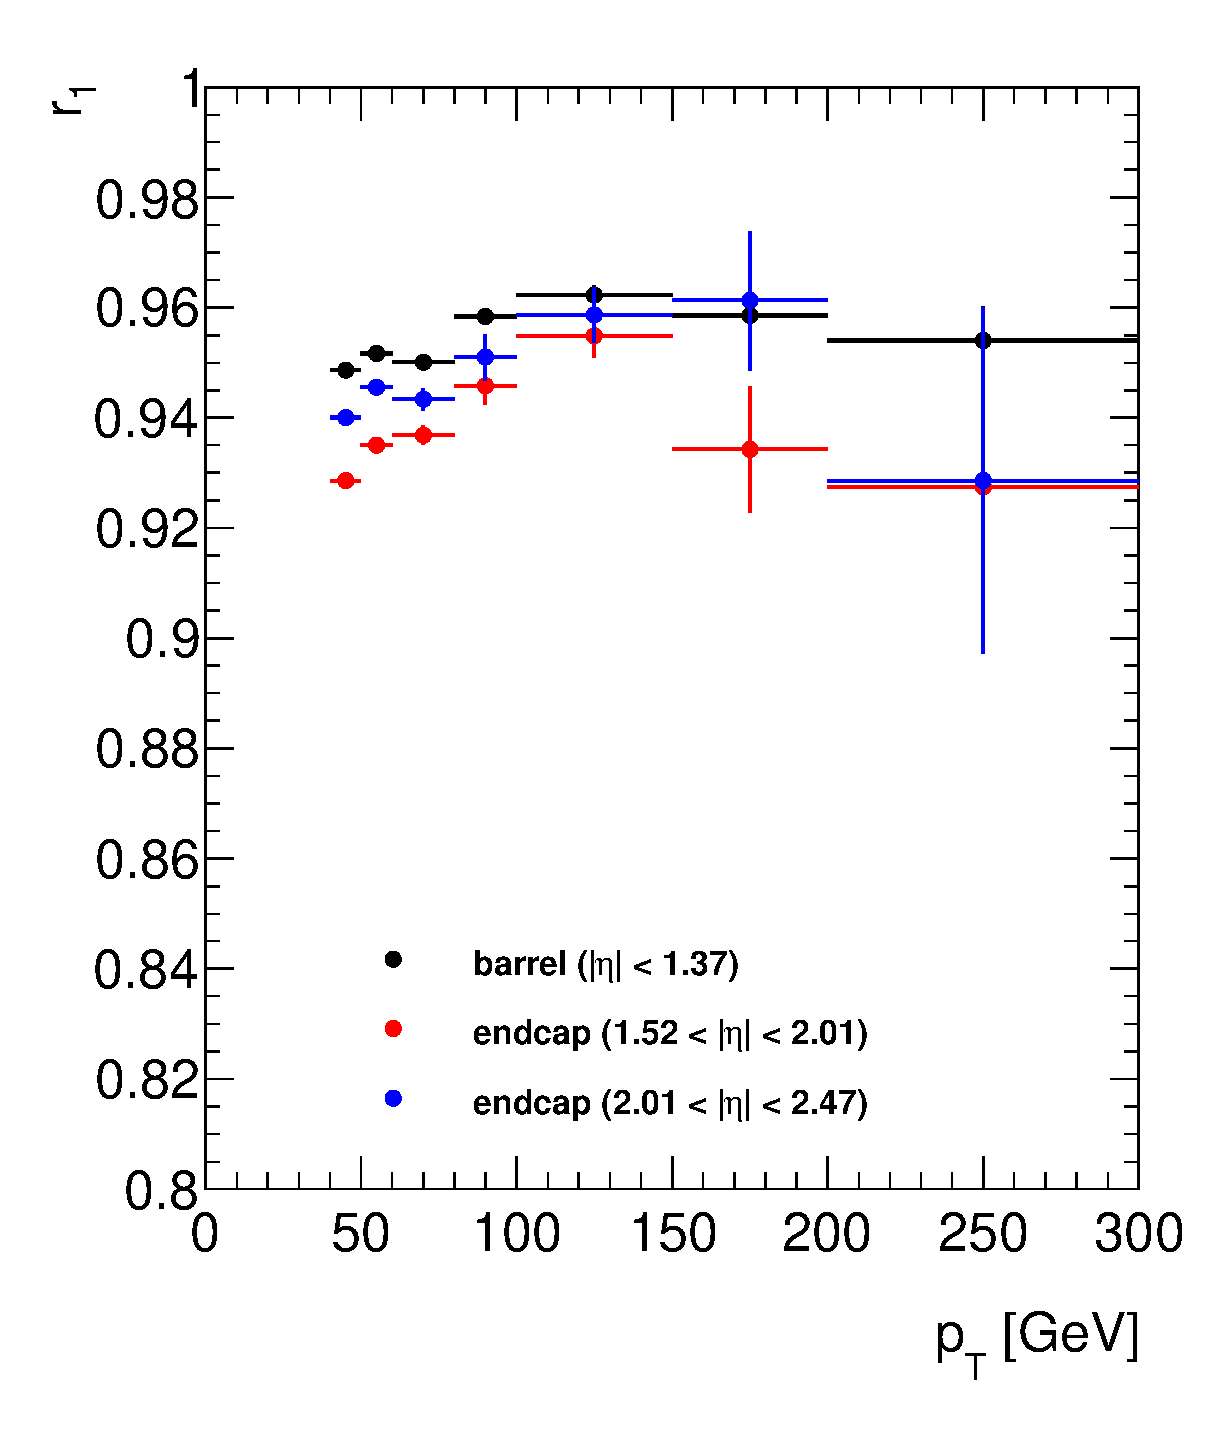
\includegraphics[scale=0.41]{images/r1.eps}
      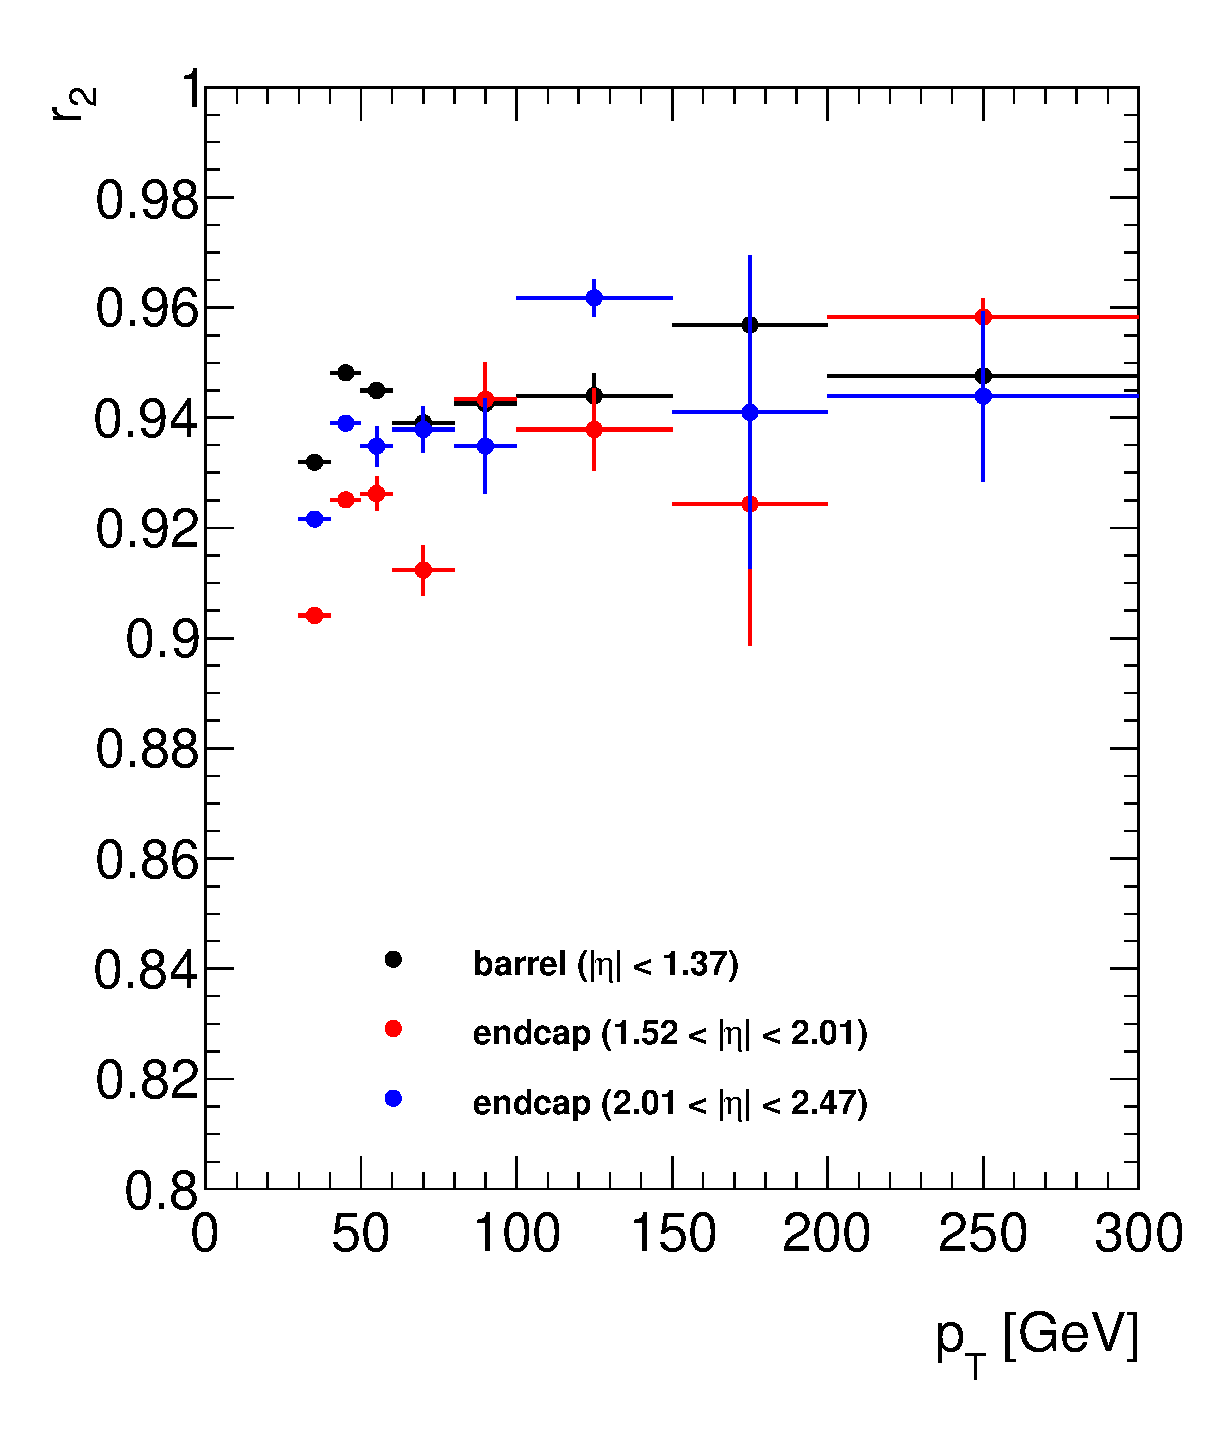
\includegraphics[scale=0.41]{images/r2.eps}
      \end{center}
   \caption{Real electron efficiencies obtained from Drell-Yan MC and binned in $p_{T}$ and three coarse $\eta$ bins covering the barrel and two endcap regions. Efficiencies for leading electrons are shown on the left while those for subleading electron are on the right.}
   \label{fig:realEff}
   \end{figure}



\subsection{Fake electron rate estimation}

The default method selected for analysing the fake rates is a single object method selection on the jet stream data. This gives the main advantage of more statistics and a higher energy reach compared to methods such as using tag and probe on the egamma stream data.
An array of triggers are used for selecting suitable events based on the single jet trigger EF\_jX\_a4chad (where X = 25, 35, 45, 55, 80, 110, 145, 180, 220, 280, 360). Events are associated to groups with the lowest trigger threshold they pass as each trigger has a different prescale. Objects are selected with the AntiKt4TopoEMJets algorithm and then matched to objects in the egamma stream with a $\Delta R~<~0.1$. Objects also have to pass the medium jet-cleaning criteria (define this). Two further steps are taken to suppress real electrons from W decays and real Drell-Yan events. A veto of $E_{Tmiss}~>~25~GeV$ is introduced to combat the former while events with two medium++ or loose++ electrons with $|m_{tag~\&~probe}-91~GeV|~<~20~GeV$ are vetoed to counter the real Drell-Yan.

The fake rate is then defined as Eq.~\ref{eq:fakeRate} $f~=~N^{fake}_{tight}/N^{fake}_{loose}$ with distributions selected using the standard event selection on the matched egamma objects.
Due to the different prescales of each trigger a separate set of fake rates are calculated for each trigger, these are then combined as a weighted average of all fake rates. Fig. \ref{fig:fakeRates} shows the distribution of fake rates for leading and subleading fakes which are distributed between 3 - $20\%$.

   \begin{figure}[h]
      \begin{center}
      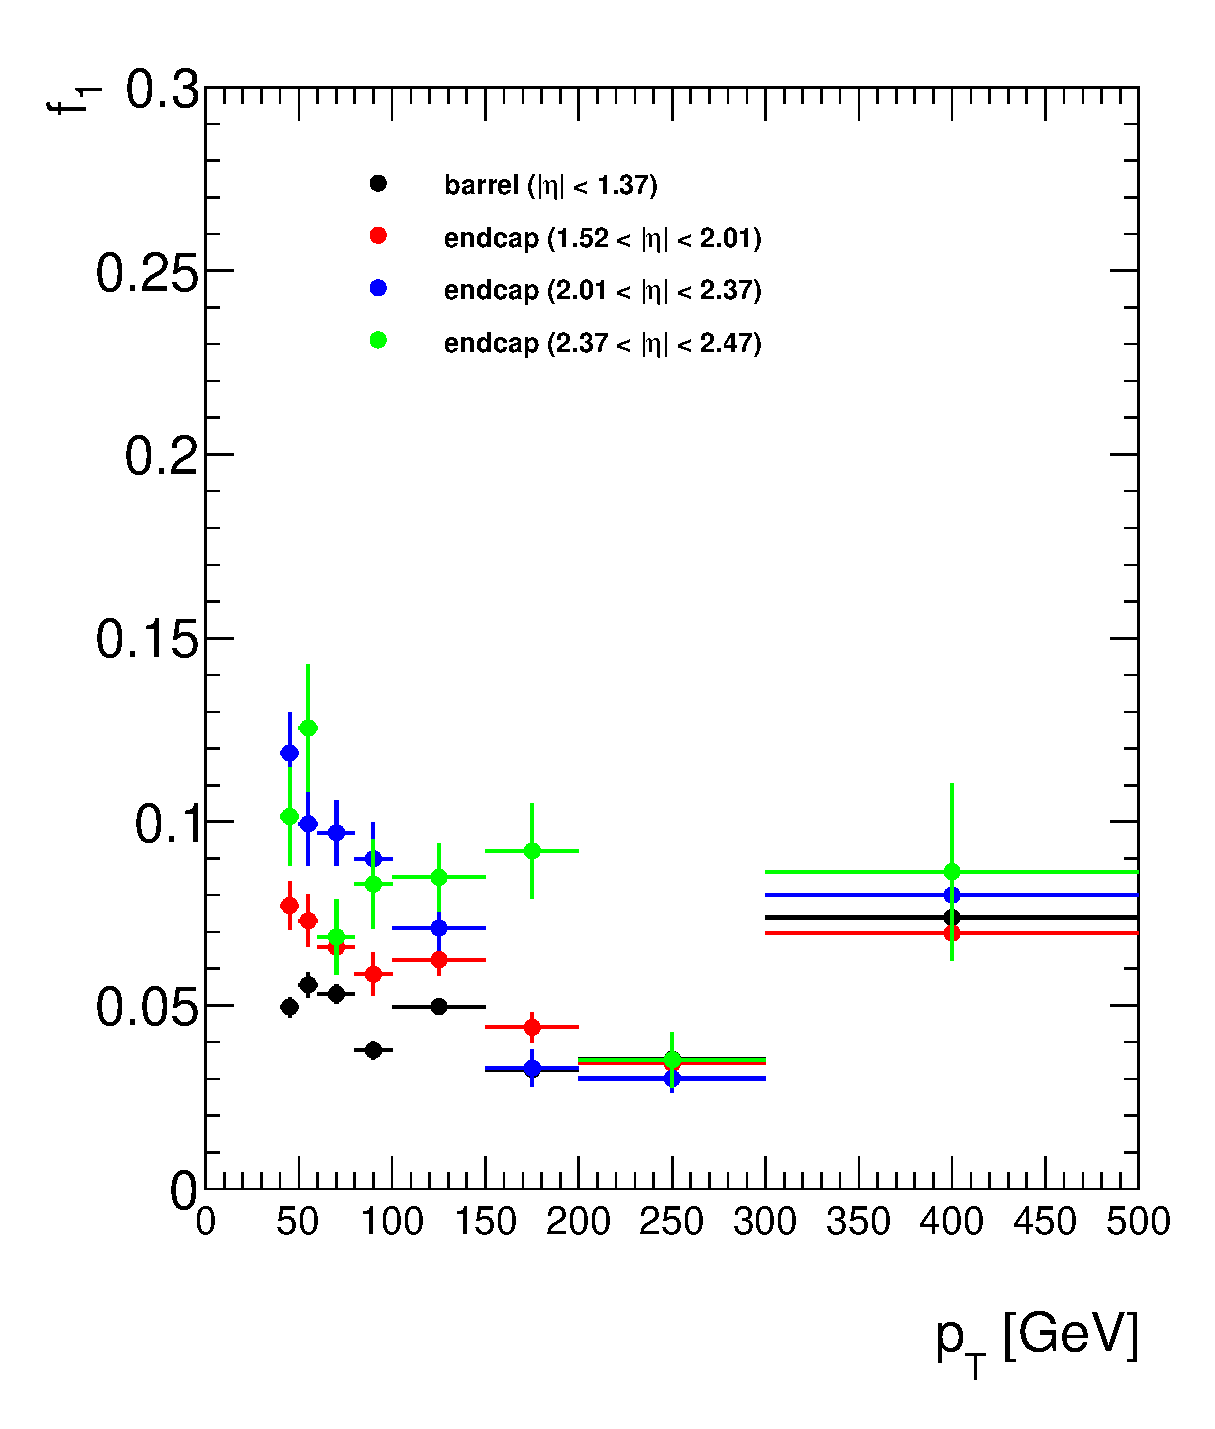
\includegraphics[scale=0.41]{images/f1.eps}
      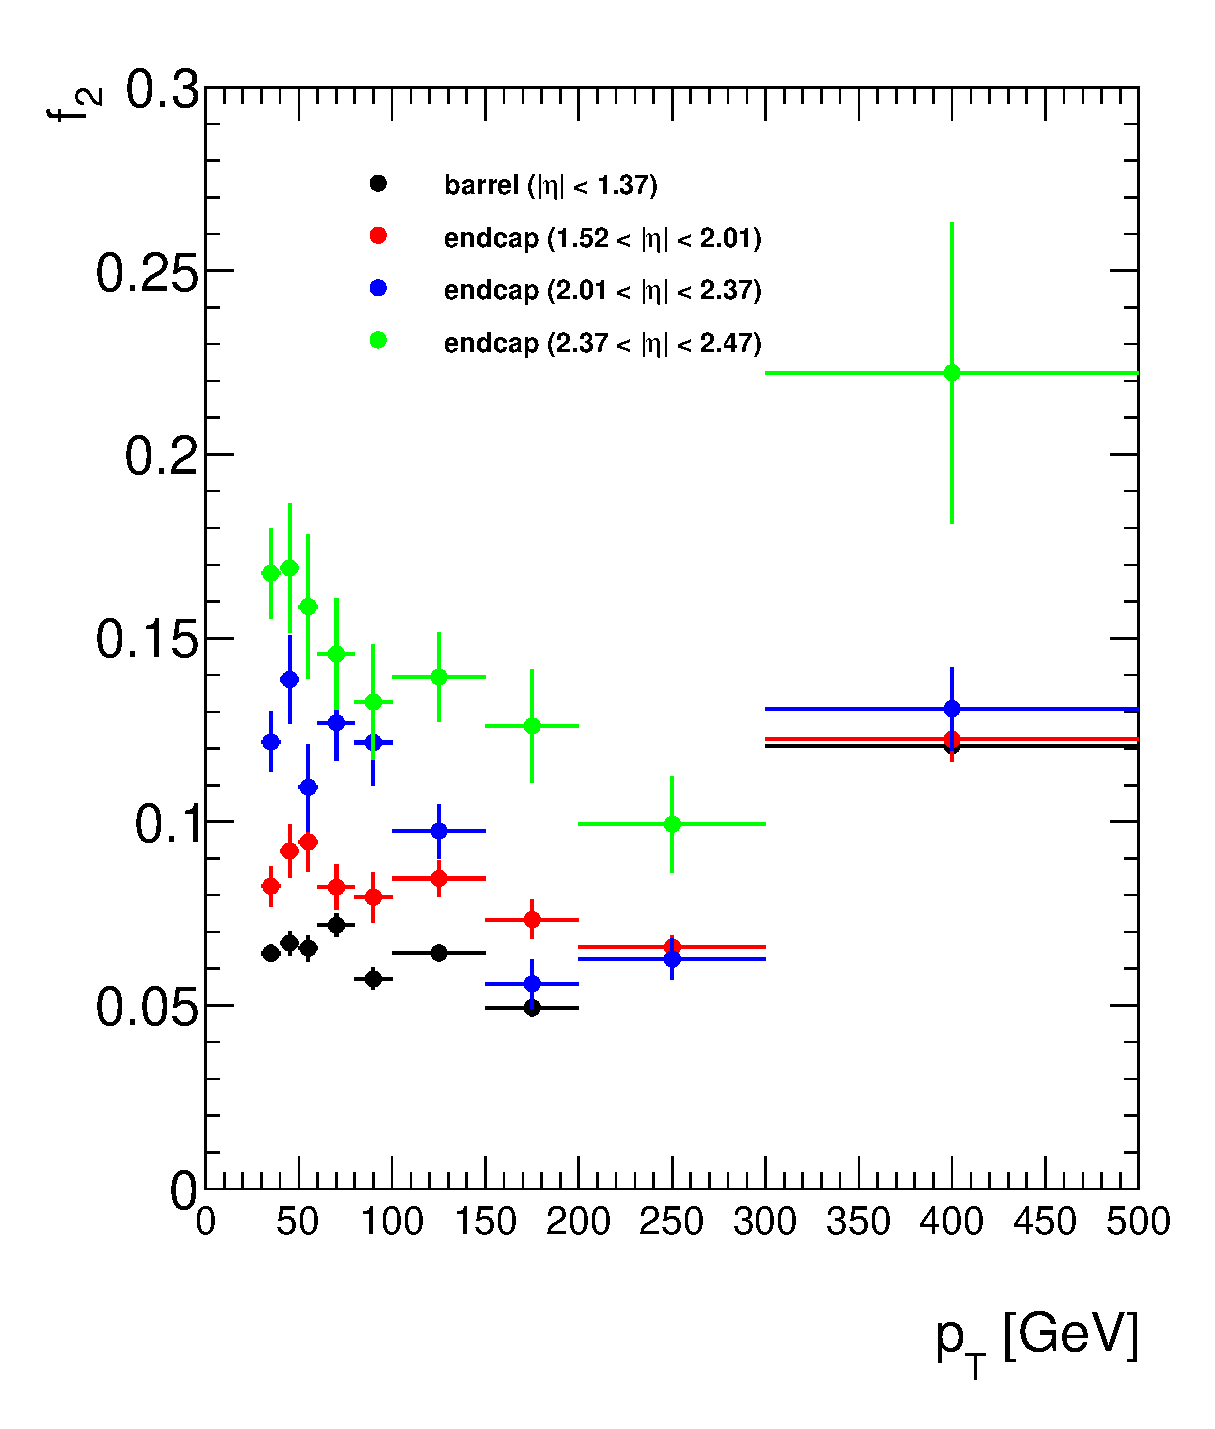
\includegraphics[scale=0.41]{images/f2.eps}
      \end{center}
   \caption{Fake rates obtained from data and binned in $p_{T}$ and four coarse $\eta$ bins covering the barrel and three endcap regions. Fake rates for leading electrons are shown on the left while those for subleading electron are on the right.}
   \label{fig:fakeRates}
   \end{figure}




\subsection{Properties of Multi-Jet Background}

In order to compose the final sample events are organised by the distributions $N_{TT}$, $N_{TL}$, $N_{LT}$ or $N_{LL}$ and weights are applied according to each electrons $p_{T}$, $\eta$ with respect to Eq.~\ref{eq:mainFakeResult} and the corresponding efficiencies and fake rates. 
Fig. \ref{fig:N_dist} shows these distributions before the efficiencies and fake rates are applied to weight to the final background prediction. In addition to these steps an extra fit is then applied at low invariant mass due to contamination due to the Z boson peak. This method is not suited to predicting the Multi-Jet background in the Z boson peak region and so a fit is obtained between 120 GeV and 400 GeV and stitched from 110 GeV and bellow. This gives a good estimate to the integral in this region for use in scaling MC's to luminosity but is not predicted to be good at predicting other variables in this region. At high-mass statistics of the sample decline and so an additional fit is made a high mass with the lower edge of the fit varied between 425 and 600 GeV and the upper edge from 700 to 1200 GeV, with the stitching point at 500 GeV.

   \begin{figure}[h]
      \begin{center}
      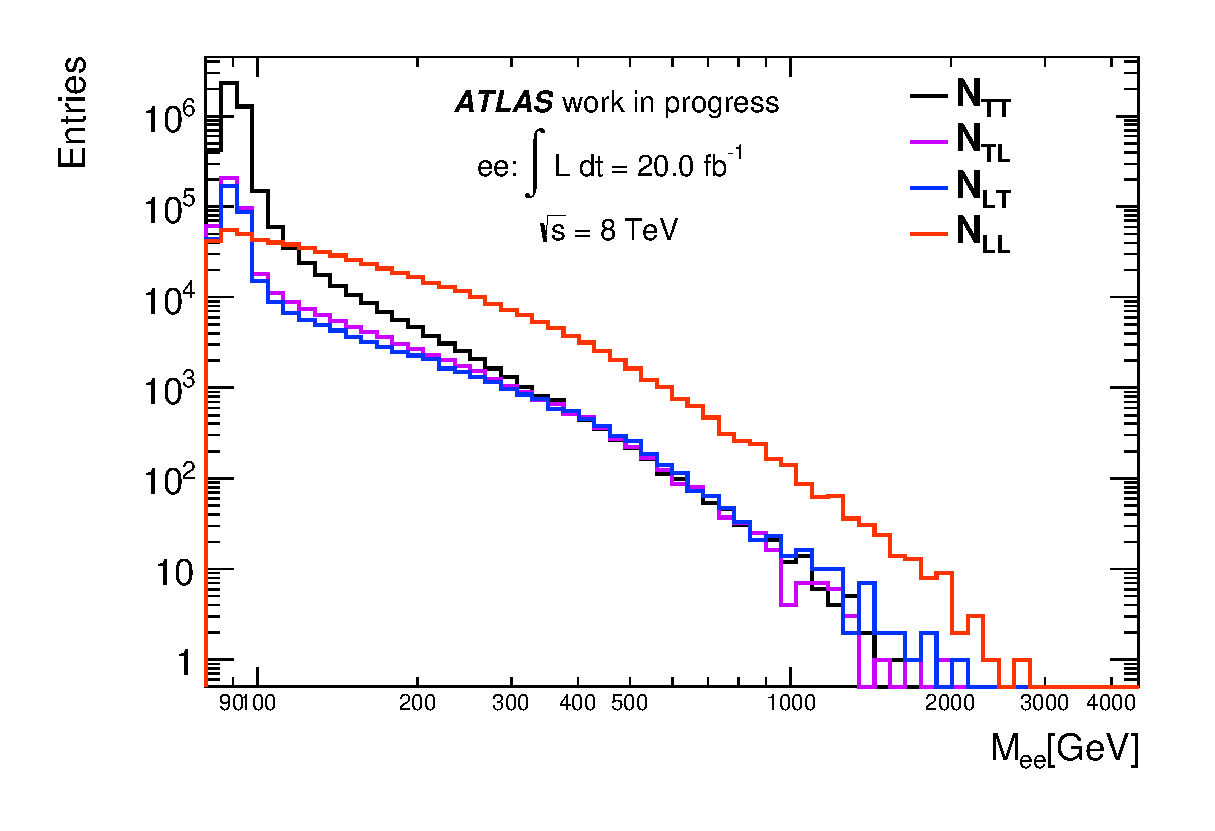
\includegraphics[scale=0.8]{images/N_distributions.eps}
      \end{center}
   \caption{Distribution of $N_{TT}$, $N_{TL}$, $N_{LT}$ and $N_{LL}$ from data with no weightings applied.}
   \label{fig:N_dist}
   \end{figure}






\subsection{Other methods and estimation of Error}
   \label{sec:MJerror}


Two other methods and variations upon them were used to test the validity of this method as well as estimate the systematic error of this background estimates procedure. These two methods are both tag and probe measurements on either the jet stream of data, or the egamma stream where the method is more an ``inverse'' tag and probe with the selection of a tag with high probability of being a jet. Variations are also made on the method by assuming $r_{1}$ and $r_{2} = 1.0$ in all cases as well as changing the definition of loose but fail tight. These variations simplify the equations slightly but the method remains the same. Fig.~\ref{fig:ff_bkg_variation} shows all of these variations compared to the default method used to obtain the estimation. This figure then gives us a good estimate to the systematic uncertainty of the multi-jet estimate which has been chosen to be a flat $20\%$.

   \begin{figure}[h]
      \begin{center}
      \includegraphics[scale=1,trim={3cm 5.5cm 3cm 14cm},clip]{images/ff_bkg_variation.ps}
      \end{center}
   \caption{Ratio of the final background estimate of all method variations to the default method. The ratio starts at 116 GeV and ends at 1500 GeV. Source: resonant support note, will not be able to use this. (NOT MADE BY ME!!!)}
   \label{fig:ff_bkg_variation}
   \end{figure}











